% questions.tex —— 2012 年·天津卷·理科 · 题目内容片段（无答案）
% 由 tools/generate_projects.py 依来源总账自 2012/2012_数学真题_天津理_试题.md 生成，勿手改（改源 MD 后重跑）

\gkpart{一、选择题}

\begin{question}
\gkti{1}$\mathrm i$ 是虚数单位，复数 $\dfrac{7-\mathrm i}{3+\mathrm i}=$\mbox{（　　）}

（A）$2+\mathrm i$；（B）$2-\mathrm i$；（C）$-2+\mathrm i$；（D）$-2-\mathrm i$。

\end{question}
\begin{question}
\gkti{2}设 $\varphi\in\mathbf R$，则“$\varphi=0$”是“$f(x)=\cos(x+\varphi)$（$x\in\mathbf R$）为偶函数”的\mbox{（　　）}

（A）充分而不必要条件；（B）必要而不充分条件；（C）充分必要条件；（D）既不充分也不必要条件。

\Needspace{0.4\textheight}
\end{question}
\begin{question}
\gkti{3}阅读如图所示的程序框图，运行相应的程序，当输入 $x$ 的值为 $-25$ 时，输出 $x$ 的值为\mbox{（　　）}
\nopagebreak[4]
\begin{center}% 2012 年天津卷理科第 3 题：输出 x 的程序框图。
% 来源 PDF：普通高考/2012/2012天津理.pdf，第 1 页（印面 775）左栏。
% 流程：开始 → 输入 x → |x|>1? 是：x=√|x|−1，回到判断；否：x=2x+1 → 输出 x → 结束。
\begin{tikzpicture}[semithick, >=Stealth,
  block/.style={draw, minimum width=3.0cm, minimum height=0.62cm, align=center},
  dec/.style={draw, diamond, aspect=2.6, inner sep=1pt, align=center},
  term/.style={draw, rounded corners=6pt, minimum width=1.5cm, minimum height=0.52cm},
  io/.style={draw, trapezium, trapezium left angle=70, trapezium right angle=110,
             minimum width=2.2cm, minimum height=0.58cm},
  arr/.style={->}]
  \node (start) [term] at (0,7.2) {开始};
  \node (input) [io]   at (0,6.25) {输入 $x$};
  \node (dec)   [dec]  at (0,5.05) {$|x|>1$?};
  \node (sq)    [block] at (0,3.7) {$x=\sqrt{|x|}-1$};
  \node (lin)   [block] at (0,2.1) {$x=2x+1$};
  \node (out)   [io]   at (0,1.05) {输出 $x$};
  \node (end)   [term] at (0,0.05) {结束};
  \draw[arr] (start) -- (input);
  \draw[arr] (input) -- (dec);
  \draw[arr] (dec) -- node[right] {是} (sq);
  \draw[arr] (sq.north west) -- (-2.1,3.7) |- (0,5.75);
  \draw[arr] (dec.east) -| node[pos=0.25, above] {否} (2.3,2.1) -- (lin.east);
  \draw[arr] (lin) -- (out);
  \draw[arr] (out) -- (end);
\end{tikzpicture}
\end{center}
\nopagebreak[4]
（A）$-1$；（B）$1$；（C）$3$；（D）$9$。

\end{question}
\begin{question}
\gkti{4}函数 $f(x)=2^x+x^3-2$ 在区间 $(0,1)$ 内的零点个数是\mbox{（　　）}

（A）$0$；（B）$1$；（C）$2$；（D）$3$。

\end{question}
\begin{question}
\gkti{5}在 $\left(2x^2-\dfrac1x\right)^5$ 的二项展开式中，$x$ 的系数为\mbox{（　　）}

（A）$10$；（B）$-10$；（C）$40$；（D）$-40$。

\end{question}
\begin{question}
\gkti{6}在 $\triangle ABC$ 中，内角 $A$，$B$，$C$ 所对的边分别是 $a$，$b$，$c$，已知 $8b=5c$，$C=2B$，则 $\cos C=$\mbox{（　　）}

（A）$\dfrac7{25}$；（B）$-\dfrac7{25}$；（C）$\pm\dfrac7{25}$；（D）$\dfrac{24}{25}$。

\end{question}
\begin{question}
\gkti{7}已知 $\triangle ABC$ 为等边三角形，$AB=2$，设点 $P$，$Q$ 满足 $\overrightarrow{AP}=\lambda\overrightarrow{AB}$，$\overrightarrow{AQ}=(1-\lambda)\overrightarrow{AC}$，$\lambda\in\mathbf R$，若 $\overrightarrow{BQ}\cdot\overrightarrow{CP}=-\dfrac32$，则 $\lambda=$\mbox{（　　）}

（A）$\dfrac12$；（B）$\dfrac{1\pm\sqrt2}2$；（C）$\dfrac{1\pm\sqrt{10}}2$；（D）$\dfrac{-3\pm2\sqrt2}2$。

\end{question}
\begin{question}
\gkti{8}设 $m$，$n\in\mathbf R$，若直线 $(m+1)x+(n+1)y-2=0$ 与圆 $(x-1)^2+(y-1)^2=1$ 相切，则 $m+n$ 的取值范围是\mbox{（　　）}

（A）$[1-\sqrt3,1+\sqrt3]$；（B）$(-\infty,1-\sqrt3]\cup[1+\sqrt3,+\infty)$；（C）$[2-2\sqrt2,2+2\sqrt2]$；（D）$(-\infty,2-2\sqrt2]\cup[2+2\sqrt2,+\infty)$。

\end{question}
\gkpart{二、填空题}

\begin{question}
\gkti{9}某地区有小学 $150$ 所，中学 $75$ 所，大学 $25$ 所。现采用分层抽样的方法从这些学校中抽取 $30$ 所学校对学生进行视力调查，应从小学中抽取\gkblank{}所学校，中学中抽取\gkblank{}所学校。

\Needspace{0.4\textheight}
\end{question}
\begin{question}
\gkti{10}一个几何体的三视图如图所示（单位：$\mathrm m$），则该几何体的体积为\gkblank{}$\mathrm m^3$。
\nopagebreak[4]
\begin{center}% 2012 年天津卷理科第 10 题：两个球与一个长方体的三视图（单位：m）。
% 来源 PDF：普通高考/2012/2012天津理.pdf，第 1 页（印面 775）右栏。
% 球半径 3/2；长方体长 6、宽 3、高 1，置于两球上方。
\begin{tikzpicture}[scale=0.72, semithick,
  dim/.style={<->, >=Stealth, thin},
  lab/.style={font=\small}]
  % ---------- 正视图 ----------
  \begin{scope}
    \draw (0,3) rectangle (6,4);
    \draw (1.5,1.5) circle (1.5);
    \draw (4.5,1.5) circle (1.5);
    \draw[->] (1.5,1.5) -- ++(1.06,1.06);
    \node at (2.30,1.92) {$\frac32$};
    \draw[->] (4.5,1.5) -- ++(1.06,1.06);
    \node at (5.30,1.92) {$\frac32$};
    \draw[dim] (0,4.45) -- (6,4.45);
    \node[above] at (3,4.45) {6};
    \draw[dim] (6.5,3) -- (6.5,4);
    \node[right] at (6.5,3.5) {1};
    \node[below] at (3,-0.55) {正视图};
  \end{scope}
  % ---------- 侧视图 ----------
  \begin{scope}[shift={(10.0,0)}]
    \draw (0,3) rectangle (3,4);
    \draw (1.5,1.5) circle (1.5);
    \draw[dim] (0,4.45) -- (3,4.45);
    \node[above] at (1.5,4.45) {3};
    \node[below] at (1.5,-0.55) {侧视图};
  \end{scope}
  % ---------- 俯视图 ----------
  \begin{scope}[shift={(0.8,-4.7)}]
    \draw (0,0) rectangle (6,3);
    \draw[dashed] (1.5,1.5) circle (1.5);
    \draw[dashed] (4.5,1.5) circle (1.5);
    \draw[dim] (6.55,0) -- (6.55,3);
    \node[right] at (6.55,1.5) {3};
    \node[below] at (3,-0.55) {俯视图};
  \end{scope}
\end{tikzpicture}
\end{center}
\nopagebreak[4]
\end{question}
\begin{question}
\gkti{11}已知集合 $A=\{x\in\mathbf R\mid|x+2|<3\}$，集合 $B=\{x\in\mathbf R\mid(x-m)(x-2)<0\}$，且 $A\cap B=(-1,n)$，则 $m=$\gkblank{}，$n=$\gkblank{}。

\end{question}
\begin{question}
\gkti{12}已知抛物线的参数方程为 $\begin{cases}x=2pt^2,\\y=2pt,\end{cases}$（$t$ 为参数），其中 $p>0$，焦点为 $F$，准线为 $l$，过抛物线上一点 $M$ 作 $l$ 的垂线，垂足为 $E$，若 $|EF|=|MF|$，点 $M$ 的横坐标是 $3$，则 $p=$\gkblank{}。

\Needspace{0.4\textheight}
\end{question}
\begin{question}
\gkti{13}如图，已知 $AB$ 和 $AC$ 是圆的两条弦，过点 $B$ 作圆的切线与 $AC$ 的延长线相交于点 $D$。过点 $C$ 作 $BD$ 的平行线与圆相交于点 $E$，与 $AB$ 相交于点 $F$，$AF=3$，$FB=1$，$EF=\dfrac32$，则线段 $CD$ 的长为\gkblank{}。
\nopagebreak[4]
\begin{center}% 2012 年天津卷理科第 13 题：圆的两条弦 AB、AC，B 处切线与 AC 延长线交于 D，
% CE∥BD 交圆于 E、交 AB 于 F。
% 来源 PDF：普通高考/2012/2012天津理.pdf，第 1 页（印面 775）右栏。
% 按 AF=3、FB=1、EF=3/2 的实际比例作图：A(0,0)，C(4,0)，D(16/3,0)，B(3.5,−1.936)，
% 圆心 (2,−0.516)，半径 2.066；E 为直线 FC 与圆的另一交点（F 在 C、E 之间）。
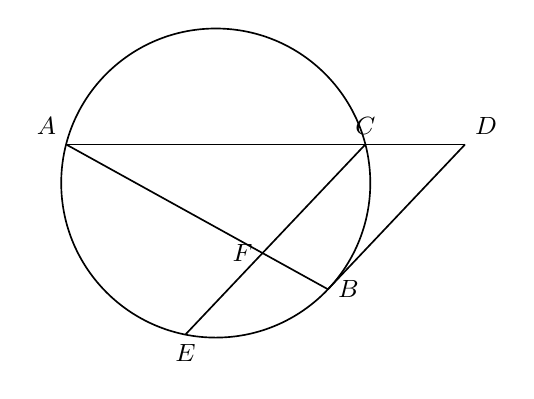
\begin{tikzpicture}[scale=0.95, semithick, font=\small]
  \coordinate (A) at (0,0);
  \coordinate (C) at (4,0);
  \coordinate (D) at (5.333,0);
  \coordinate (B) at (3.5,-1.936);
  \coordinate (F) at (2.625,-1.452);
  \coordinate (E) at (1.594,-2.542);
  \coordinate (O) at (2,-0.516);
  \draw (O) circle (2.066);
  \draw (A) -- (B);
  \draw (A) -- (C);
  \draw (C) -- (D);
  \draw (B) -- (D);
  \draw (E) -- (C);
  \node[above left] at (A) {$A$};
  \node[above] at (C) {$C$};
  \node[above right] at (D) {$D$};
  \node[right] at (B) {$B$};
  \node[left] at (F) {$F$};
  \node[below] at (E) {$E$};
\end{tikzpicture}
\end{center}
\nopagebreak[4]
\end{question}
\begin{question}
\gkti{14}已知函数 $y=\dfrac{|x^2-1|}{x-1}$ 的图象与函数 $y=kx-2$ 的图象恰有两个交点，则实数 $k$ 的取值范围是\gkblank{}。

\end{question}
\gkpart{三、解答题}

\begin{question}
\gkti{15}已知函数 $f(x)=\sin\left(2x+\dfrac\pi3\right)+\sin\left(2x-\dfrac\pi3\right)+2\cos^2x-1$，$x\in\mathbf R$。

（1） 求函数 $f(x)$ 的最小正周期；

（2） 求函数 $f(x)$ 在区间 $\left[-\dfrac\pi4,\dfrac\pi4\right]$ 上的最大值和最小值。

\end{question}
\begin{question}
\gkti{16}有 $4$ 个人去参加某娱乐活动，该活动有甲、乙两个游戏可供参加者选择。为增加趣味性，约定：每个人通过掷一枚质地均匀的骰子决定自己去参加哪个游戏，掷出点数为 $1$ 或 $2$ 的人去参加甲游戏，掷出点数大于 $2$ 的人去参加乙游戏。

（1） 求这 $4$ 个人中恰有 $2$ 人去参加甲游戏的概率；

（2） 求这 $4$ 个人中去参加甲游戏的人数大于去参加乙游戏的人数的概率；

（3） 用 $X$，$Y$ 分别表示这 $4$ 个人中去参加甲、乙游戏的人数，记 $\xi=|X-Y|$，求随机变量 $\xi$ 的分布列与数学期望 $E\xi$。

\Needspace{0.4\textheight}
\end{question}
\begin{question}
\gkti{17}如图，在四棱锥 $P-ABCD$ 中，$PA\perp$ 平面 $ABCD$，$AC\perp AD$，$AB\perp BC$，$\angle BAC=45^\circ$，$PA=AD=2$，$AC=1$。

（1） 证明 $PC\perp AD$；

（2） 求二面角 $A-PC-D$ 的正弦值；

（3） 设 $E$ 为棱 $PA$ 上的点，满足异面直线 $BE$ 与 $CD$ 所成的角为 $30^\circ$，求 $AE$ 的长。
\nopagebreak[4]
\begin{center}% 2012 年天津卷理科第 17 题：四棱锥 P-ABCD，PA⊥平面 ABCD。
% 来源 PDF：普通高考/2012/2012天津理.pdf，第 2 页（印面 776）第 1 栏。
% 图中 A 在底面前部居中，B 在其右后，C 在最右，D 在左后；虚线为被遮挡的棱 PA、PB、AD、AB、BC 与对角线 AC。
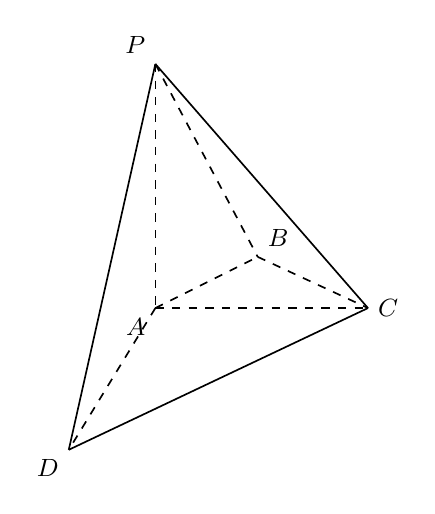
\begin{tikzpicture}[scale=1.0, semithick, font=\small]
  \coordinate (P) at (0.2,3.3);
  \coordinate (A) at (0.2,0.2);
  \coordinate (B) at (1.5,0.85);
  \coordinate (C) at (2.9,0.2);
  \coordinate (D) at (-0.9,-1.6);
  \draw (P) -- (C);
  \draw (P) -- (D);
  \draw (D) -- (C);
  \draw[dashed] (P) -- (A);
  \draw[dashed] (P) -- (B);
  \draw[dashed] (A) -- (B);
  \draw[dashed] (B) -- (C);
  \draw[dashed] (A) -- (C);
  \draw[dashed] (A) -- (D);
  \node[above left] at (P) {$P$};
  \node[below left] at (A) {$A$};
  \node[above right] at (B) {$B$};
  \node[right] at (C) {$C$};
  \node[below left] at (D) {$D$};
\end{tikzpicture}
\end{center}
\nopagebreak[4]
\end{question}
\begin{question}
\gkti{18}已知 $\{a_n\}$ 是等差数列，其前 $n$ 项和为 $S_n$，$\{b_n\}$ 是等比数列，且 $a_1=b_1=2$，$a_4+b_4=27$，$S_4-b_4=10$。

（1） 求数列 $\{a_n\}$ 与 $\{b_n\}$ 的通项公式；

（2） 记 $T_n=a_nb_1+a_{n-1}b_2+\cdots+a_1b_n$，$n\in\mathbf N^*$，证明 $T_n+12=-2a_n+10b_n$（$n\in\mathbf N^*$）。

\end{question}
\begin{question}
\gkti{19}设椭圆 $\dfrac{x^2}{a^2}+\dfrac{y^2}{b^2}=1$（$a>b>0$）的左、右顶点分别为 $A$，$B$，点 $P$ 在椭圆上且异于 $A$，$B$ 两点，$O$ 为坐标原点。

（1） 若直线 $AP$ 与 $BP$ 的斜率之积为 $-\dfrac12$，求椭圆的离心率；

（2） 若 $|AP|=|OA|$，证明直线 $OP$ 的斜率 $k$ 满足 $|k|>\sqrt3$。

\end{question}
\begin{question}
\gkti{20}已知函数 $f(x)=x-\ln(x+a)$ 的最小值为 $0$，其中 $a>0$。

（1） 求 $a$ 的值；

（2） 若对任意的 $x\in[0,+\infty)$，有 $f(x)\leqslant kx^2$ 成立，求实数 $k$ 的最小值；

（3） 证明：$\displaystyle\sum_{i=1}^{n}\frac{2}{2i-1}-\ln(2n+1)<2$（$n\in\mathbf N^*$）。

\end{question}